% !TEX root = ../main.tex

\chapter{Method}
\label{ch:method}

\section{Benchmarks in Reinforcement Learning}
\label{sec:benchmarks}
When developing a novel algorithm, it is important to compare our results with existing models. For this evaluation, we need standard benchmark problems. These are a set of standard optimization problems. OpenAI Gym is a toolkit created for exactly this scenario. As mentioned in Section~\ref{sec:gym}, it contains a collection of benchmark problems with various levels of difficulty. However, not all benchmark problems are meaningful for the evaluation of an algorithm. If a problem is too trivial to solve, the results do not reflect the quality of the model adequately. We do not need to put a large amount of effort into the creation of a complex model for an easy-to-solve task.

In the paper \emph{Analyzing Reinforcement Learning Benchmarks with Random Weight Guessing} (\cite{oller_analyzing_2020}), the authors analyze and visualize the complexity of standard RL benchmarks based on score distribution. They tested their approach on the five Classic Control benchmark problems from the OpenAI Gym interface: \verb|CartPole|, \verb|Acrobot|, \verb|Pendulum|, \verb|MountainCar|, and \verb|MountainCarCon-| \verb|tinuous|. Given an RL environment, the authors conducted a fixed series of experiments. For these experiments, they used three neural network architectures ($N_{architectures}=3$): a network without any hidden layers (0 HL, 0 HU), a network with a single hidden layer of 4 units (1 HL, 4 HU), and a network with two hidden layers of 4 units each (2 HL, 4 HU). With these, they cover a variety of network models that are suited to solve the given tasks. The evaluation of the benchmark problems should be as objective as possible and should not include bias in the data. To achieve this, the authors did not include any learning opportunities for the network models. Instead, they chose the network weights i.i.d. from the standard normal distribution $\mathcal{N}(0,1)$ with Random Weight Guessing (RWG). This approach assures randomness and no directed learning. The goal of the paper was not to further analyze the network models but to investigate the benchmark problems themselves. With this in mind, they initialized $10^4$ samples ($N_{samples}=10^4$) with different random weights. The number of samples would be too large for a reasonable learning strategy. However, the large number of samples serves a different purpose than optimizing the results. Instead, the aim is to draw statistical conclusions. Each of these samples of a neural network represents a controller that maps observations to actions in the environment. Later in this thesis, I will explore function approximators other than neural networks representing the controller. In the paper, the authors tested the controllers for each environment during 20 independent episodes ($N_{episodes}=20$). For each episode, they saved the score in the score tensor $S$. Algorithm~\ref{alg:environment-evaluation} illustrates the procedure with pseudocode.

\begin{algorithm}
\caption{Evaluation process taken from \cite{oller_analyzing_2020}}
\begin{algorithmic}[1]
\State Initialize environment
\State Create array $S$ of size $N_{architectures} \times N_{samples} \times N_{episodes}$
\For{$n = 1,2,...,N_{samples}$}
    \State Sample NN weights randomly from $\mathcal{N}(0,1)$
    \For{$e=1,2,...,N_{episodes}$}
      \State Reset the environment
      \State Run episode with NN
      \State Store accured episode reward in $S_{a,n,e}$
    \EndFor
\EndFor
\end{algorithmic}
\label{alg:environment-evaluation}
\end{algorithm}

After the authors obtained the scores, they calculated the mean performance over all episodes from a sample and its variance. These statistics are significant insights. They can reveal how stable the network models are in completing a given task. A low mean value suggests that, in general, the network cannot complete the task. The variance gives us further insight into the score distribution. It illustrates how spread out the scores are from their respective mean score. A high value means that we have high variability. A controller is valuable if it can solve a specific task reliably and stable. Therefore, we strive for a high value for the mean and a low value for the variance. However, training a network with random weight guessing should generally not result in a stable controller. If this is the case, we can assume that the task to solve was too trivial and is not valuable for evaluation measurements. In the illustrations of the paper, the authors ranked the samples according to their mean scores. They then visualized their results with three plots: a log-scale histogram of the mean scores, a scatter plot of the sample scores over their rank, a scatter plot of score variance over the mean score.

I reproduced the results of the authors following the mentioned methodology. My findings for the environment \verb|CartPole| are displayed in Figure~\ref{fig:plots_reproduced}.
\begin{figure}[ht]
\centering
\begin{subfigure}{\textwidth}
  \centering
  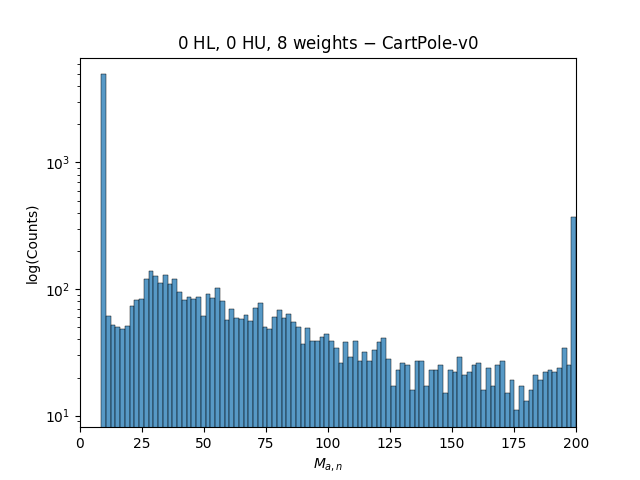
\includegraphics[width=0.329\textwidth]{reproduced_plots/HL_0_HU_0_histogram}
  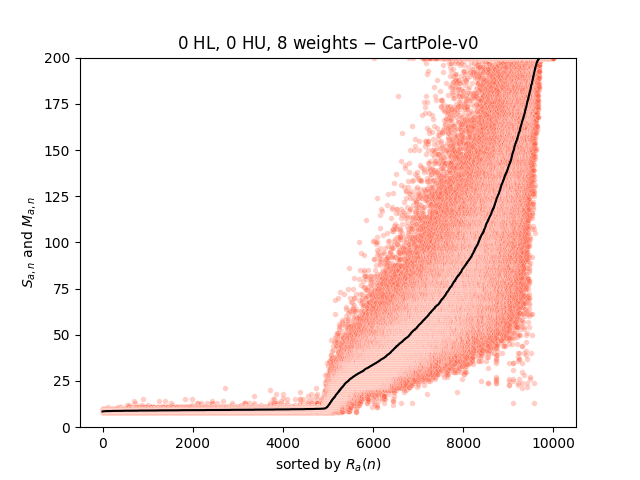
\includegraphics[width=0.329\textwidth]{reproduced_plots/HL_0_HU_0_scatter_score}
  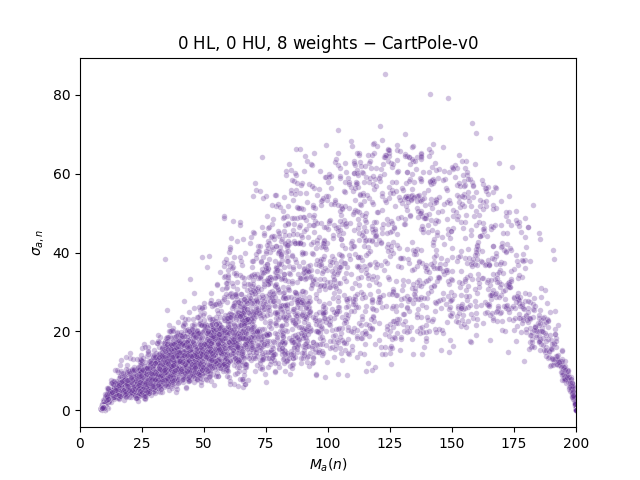
\includegraphics[width=0.329\textwidth]{reproduced_plots/HL_0_HU_0_scatter_sd}
    \caption{Results of network architecture without hidden layers}
    \label{fig:plots_reproduced_first}
\end{subfigure}
\begin{subfigure}{\textwidth}
  \centering
  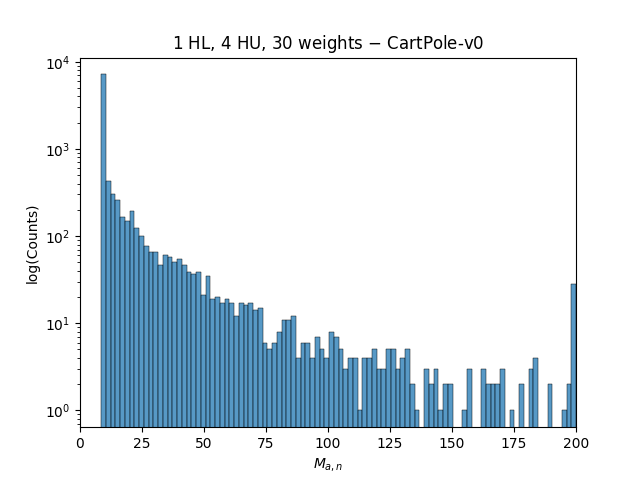
\includegraphics[width=0.329\textwidth]{reproduced_plots/HL_1_HU_4_histogram}
  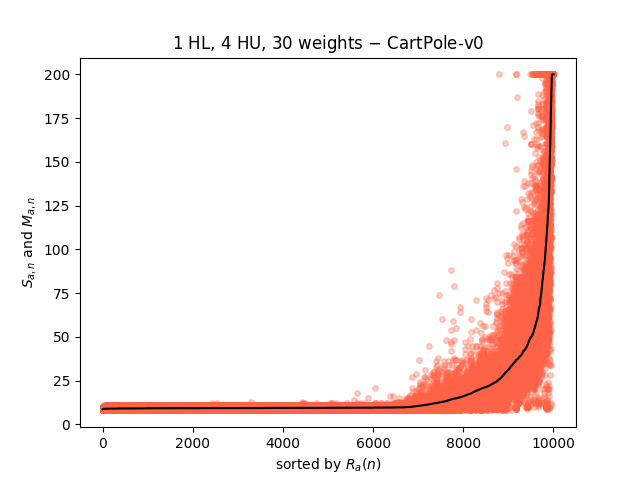
\includegraphics[width=0.329\textwidth]{reproduced_plots/HL_1_HU_4_scatter_score}
  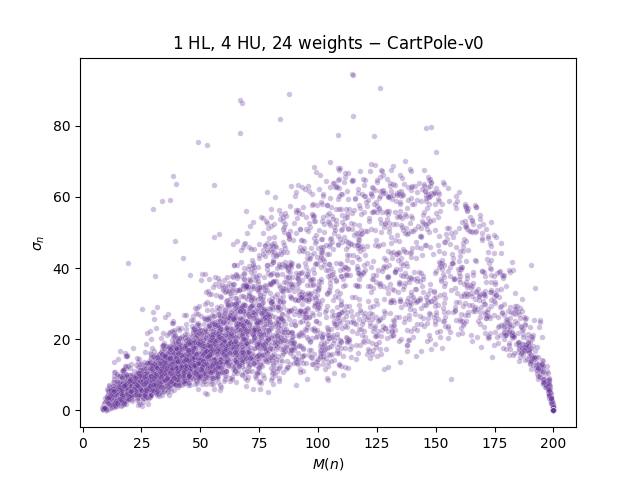
\includegraphics[width=0.329\textwidth]{reproduced_plots/HL_1_HU_4_scatter_sd}
    \caption{Results of network architecture with one hidden layer}
    \label{fig:plots_reproduced_second}
\end{subfigure}
\begin{subfigure}{\textwidth}
  \centering
  \includegraphics[width=0.329\textwidth]{reproduced_plots/HL_2_HU_4_histogram}
  \includegraphics[width=0.329\textwidth]{reproduced_plots/HL_2_HU_4_scatter_score}
  \includegraphics[width=0.329\textwidth]{reproduced_plots/HL_2_HU_4_scatter_sd}
    \caption{Results of network architecture with two hidden layers}
    \label{fig:plots_reproduced_third}
\end{subfigure}
\caption[Reproduced Plots]{
  \textbf{Results of the benchmark evaluation.}
   The plots show a log-scale histogram of the mean scores (left images), a scatter plot of the sample scores over their rank (middle images), a scatter plot of score variance over the mean score (right image). As expected with RWG, most networks were not able to solve the given task. However, there is still a significant amount of samples achieving a mean score of 200. That suggests that the environment is trivial to solve.
}
\label{fig:plots_reproduced}
\end{figure}
The plots illustrate the results for each of the three network architectures. Each row shows the histogram of the mean score values in the left image, the scatter plot of all scores over their rank in the image in the middle, and the scatter plot of the score variance over the mean score in the right image for a specific network architecture. There are few differences, but overall all network architectures deliver similar insights. The histogram plots show that the majority of networks receive a low score. Since the weights of the networks were chosen with RWG, this is rather unsurprising. But there is still a significant amount of networks that were able to achieve a high mean value or even the maximum value of 200. With a score of 200, the network was able to solve the task each episode. Therefore, the network could reliably solve the task without any learning technique involved. This should not be the case for a complex task. Furthermore, in the scatter plot in the middle, we can see that the line plot of the mean scores is a continuous increasing line without any jumps. Thus, a suited RL algorithm should generally be able to learn the task incrementally without converging into a local optimum. At the top of the scatter plot, we can see quite a few data points with a score of 200 that have a relatively low mean score. This indicates that a network that generally performs poorly can still solve the task with the right initialization conditions. Lastly, in the scatter plot on the right, we can see the distribution of the variance according to the mean value. On the left side, we have low scores of variance corresponding with a low mean value. These networks were consistently unable to achieve a high score. Without any training involved, we can expect most networks to be in this area. However, in the middle of the plot, the data points are spread out. For a high variance, the scores of a network differ highly from the mean value. Thus, we might get lucky and receive a high score depending on initialization conditions, but we might as well get a low score. These networks are inconsistent and unstable. On the right side of the scatter plot, we can see that the data points with a high mean value are mostly of low variance. Thus, to achieve a high mean value, the network needs consistency.

\subsection{Impact of Bias}
Interestingly, the usage of the bias had a relatively large impact on the performance of the network in my experiments. Without bias, the networks seem to achieve overall better scores. All plots in Figure~\ref{fig:plots_reproduced} illustrate the results without bias. For comparison, Figure~\ref{fig:comparison_bias} shows the results of a network with two hidden layers with the same configurations as before but this time including bias. As we can see, the networks with bias connections have a much lower score in general. The number of networks that can consistently solve the task also decreases significantly. In the paper, the authors noted that the probability mass of top-performers generally increases when dropping the bias connections for all tested environments. Thus, this is not an isolated observation. However, they did not investigate this behavior further as it was not the focus of their paper.
\begin{figure}[ht]
\centering
\includegraphics[width=0.329\textwidth]{with_bias_nn/HL_2_HU_4_histogram}
\includegraphics[width=0.329\textwidth]{with_bias_nn/HL_2_HU_4_scatter_score}
\includegraphics[width=0.329\textwidth]{with_bias_nn/HL_2_HU_4_scatter_sd}
\caption[Impact of Bias]{
  \textbf{Impact of bias.}
  The figures show the performance of a network with two hidden layers with the same settings as before but here we include bias. We can clearly see that the network with bias connection performs much worse than the one without.
}
\label{fig:comparison_bias}
\end{figure}
One possible explanation could be that guessing additional weights might be fatal for achieving a good score. Or in other words: the more possibilities we have to falsely guess a weight, the higher the probability to fail. To test this hypothesis, we can alter the number of weights and compare the results. With an increased number of weights, we would expect the networks to perform worse than before. However, it could also be that the number of weights is not as impactful as the complexity of the model in general. Randomly guessing the parameters of a simple model has a higher chance to result in a good (simple) model than guessing the parameters of a more complex model. The complexity of the network architecture gives an upper bound for the function that can be approximated. A network with high complexity maps into a larger search space with more complex functions. Since the size of the search space increases, there are also more possible samples that fail to solve the task. As the paper showed, a simple model is sufficient to solve these environments. A complex model is oversized for our purpose here. Thus, randomly guessing a simple model can yield a model with good performance with enough attempts. However, it is unlikely to randomly guess a complex model that performs well without any training involved. To test this hypothesis, we can increase the complexity of a network by varying the number of hidden layers or the number of neurons in a hidden layer. With increased complexity, we would expect the networks to perform worse than before.

Another interesting aspect would be to inspect the role of the bias in connection with the environments. A simple model is sufficient to solve a simple task. But what if the environment is more difficult to solve? In that case, the undersized complexity would limit us from finding an appropriate solution as the search space is not large enough for this scenario. Therefore, including bias should improve the results.

The experiments following this thought process are described in Chapter~\ref{ch:experiments}.


\todo[inline]{How much should be included here and how much in experiments/visualization? Rename section name?}

\section{OpenAI Gym Environments}
\label{sec:environments}
OpenAI Gym offers five classic control environments ready to use: \verb|CartPole|, \verb|Acrobot|, \verb|MountainCar|, \verb|MountainCarContiuous|, and \verb|Pendulum|. The initial state of each environment is stochastic. Out of all environments OpenAI Gym provides, the classic control environments are considered the easier ones to solve. Each environment holds an observation and an action space. An agent performs some action from the action space and receives an observation describing how the environment's state changed.

\subsection{CartPole}
The \verb|CartPole| environment corresponds to the pole-balancing problem formulated in \emph{Neuronlike Adaptive Elements That Can Solve Difficult Learning Control Problems} (\cite{6313077}). A pole is attached to a cart that the agent can move along a one-dimensional track. Fig.~\ref{fig:cartpole} shows two possible states of this problem. In the image on the left, the pole is perfectly balanced and upright. The right image shows the pole tilted to the left. Thus, the cart should go to the left to correct the angle of the pole.
\begin{figure}[!ht]
  \centering
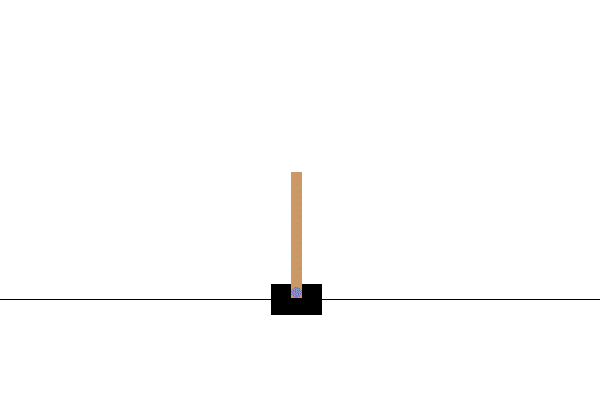
\includegraphics[width=0.4\textwidth]{cartpole} \hspace*{10mm} 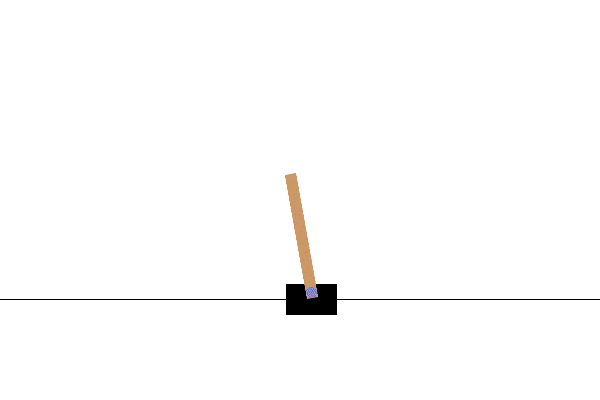
\includegraphics[width=0.4\textwidth]{cartpole_tilted}
\caption[Illustration of the environment CartPole]{
  \textbf{Illustration of the environment CartPole.}
  The image shows two possible states of the \texttt{CartPole} environment. The left image shows a perfectly balanced pole. In the right image, the pole tilts to the left.
}
\label{fig:cartpole}
\end{figure}

\paragraph*{Action Space:} The \verb|CartPole| environment accepts one action per time step and has a discrete action space of \{0, 1\}. The action indicates the direction in which we push the cart by a fixed force. The actions are described in Table~\ref{table:cartpole_act}.
\begin{table}[!ht]
  \centering
  \begin{tabular}{ |c|c| }
    \hline
    Action & Description \\
    \hline
    0 & Push cart to the left \\
    1 & Push cart to the right \\
    \hline
  \end{tabular}
  \caption[Action space of the environment CartPole]{
    \textbf{Action space of the environment CartPole.}
    Description of all possible actions for the \texttt{CartPole} environment.
  }
  \label{table:cartpole_act}
\end{table}

\paragraph*{Observation Space:} For \verb|CartPole|, we receive four observations that inform us about the position and velocity of the cart and the pole. Table~\ref{table:cartpole_obs} shows all observations with the range of the corresponding values.
\begin{table}[!ht]
  \centering
  \begin{tabular}{ |c|c|c| }
    \hline
    Observation & Min & Max \\
    \hline
    Cart Position & -4.8 & 4.8 \\
    Cart Velocity & -Inf & Inf \\
    Pole Angle & ~ -0.418 rad (-24°) & ~ 0.418 rad (24°) \\
    Pole Angular Velocity & -Inf & Inf \\
    \hline
  \end{tabular}
  \caption[Observation space of the environment CartPole]{
    \textbf{Observation space of the environment CartPole.}
    Description of all observations for the \texttt{CartPole} environment.
  }
  \label{table:cartpole_obs}
\end{table}

\paragraph*{Reward:} The goal of this task is to keep the pole upright as long as possible. Thus, we get a positive reward of +1 for each step that does not meet the termination criteria. An episode terminates when the pole angle is $\pm$12°, the cart position is $\pm$2.4, or the episode length is higher than 200 (500 for v1).

\subsection{Acrobot}
The environment \verb|Acrobot| is based on the paper \emph{Generalization in Reinforcement Learning: Successful Examples Using Sparse Coarse Coding} (\cite{NIPS1995_8f1d4362}) and the book \emph{Reinforcement Learning: An Introduction} (\cite{montague1999reinforcement}). The system contains a chain with two links, with one end of the chain fixed. The goal is to swing the free end of the chain upwards until reaching a certain height. Fig~\ref{fig:acrobot} shows in the left image one possible state for this problem with the fixed height indicated by a horizontal line. The right image of the figure illustrates one possible state that reached the target height.
\begin{figure}[!ht]
  \centering
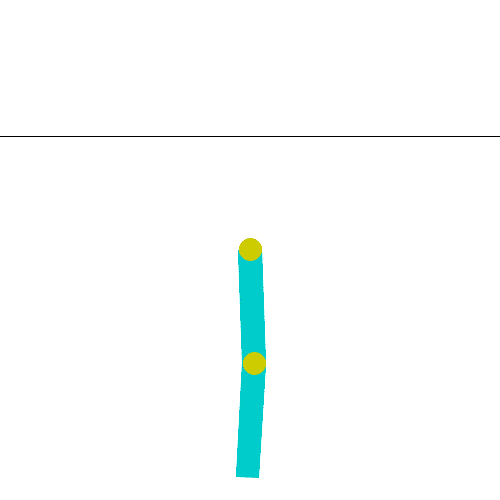
\includegraphics[width=0.4\textwidth]{acrobot} \hspace*{10mm} 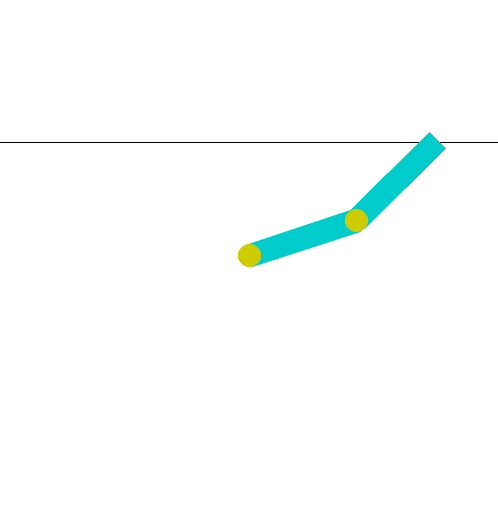
\includegraphics[width=0.4\textwidth]{acrobot_solved}
\caption[Illustration of the environment Acrobot]{
  \textbf{Illustration of the environment Acrobot.}
  The image on the left shows one possible state of the environment \texttt{Acrobot}. The image on the right shows one possibility of reaching the target height.
}
\label{fig:acrobot}
\end{figure}

\paragraph*{Action Space:} For \verb|Acrobot|, the action space is discrete and deterministic, representing the torque applied to the joint between the two links, including the loose end. Table~\ref{table:acrobot_act} shows a description of all possible actions.
\begin{table}[!ht]
  \centering
  \begin{tabular}{ |c|c|c| }
    \hline
    Action & Description & Unit \\
    \hline
    0 & apply -1 torque to the actuated joint & torque (N m) \\
    1 & apply 0 torque to the actuated joint & torque (N m) \\
    2 & apply 1 torque to the actuated joint & torque (N m) \\
    \hline
  \end{tabular}
  \caption[Action space of the environment Acrobot]{
    \textbf{Action space of the environment Acrobot.}
    Description of all possible actions for the \texttt{Acrobot} environment.
  }
  \label{table:acrobot_act}
\end{table}

\paragraph*{Observation Space:} \verb|Acrobot| returns six observations that inform us about the two rotational joint angles and their angular velocities. Table~\ref{table:acrobot_obs} contains a description for each observation. theta1 is the angle of the first joint, where an angle of 0 indicates that the first link is pointing directly downwards. theta2 is relative to the angle of the first link. An angle of 0 corresponds to having the same angle between the two links.
\begin{table}[!ht]
  \centering
  \begin{tabular}{ |c|c|c| }
    \hline
    Observation & Min & Max \\
    \hline
    Cosine of theta1 & -1 & 1 \\
    Sine of theta1 & -1 & 1 \\
    Cosine of theta2 & -1 & 1 \\
    Sine of theta2 & -1 & 1 \\
    Angular velocity of theta1 & ~ -12.567 (-4 * $\pi$) & ~ 12.567 (4 * $\pi$) \\
    Angular velocity of theta2 & ~ -28.274 (-9 * $\pi$) & ~ 28.274 (9 * $\pi$) \\
    \hline
  \end{tabular}
  \caption[Observation space of the environment Acrobot]{
    \textbf{Observation space of the environment Acrobot.}
    Description of all observations for the \texttt{Acrobot} environment.
  }
  \label{table:acrobot_obs}
\end{table}

\paragraph*{Reward:} The goal of this task is to reach the target height with as few steps as possible. Thus, each step that does not attain the goal receives a negative reward of -1. Reaching the target height results in a reward of 0. The reward threshold is -100.

\subsection{MountainCar and MountainCarContiuous}
The environments \verb|MountainCar| and \verb|MountainCarContiuous| are two different versions of the same problem. The difference between the two is that \verb|MountainCar| has a discrete action space, and \verb|MountainCarContinuous| has a continuous action space. The goal of the task is to maneuver a car up a hill to its target. To achieve this, we need to strategically accelerate the car. An agent ought to learn how to swing from left to right to reach the target. This task is rather difficult to learn since we counterintuitively need to move in the opposite direction of the target to swing up. The problem first appeared in Andrew Moore's PhD thesis \emph{Efficient memory-based learning for robot control} (\cite{moore1990efficient}). Fig~\ref{fig:mountain_car} shows one possible state in the left image and the target state of the two environments in the right image.
\begin{figure}[!ht]
  \centering
  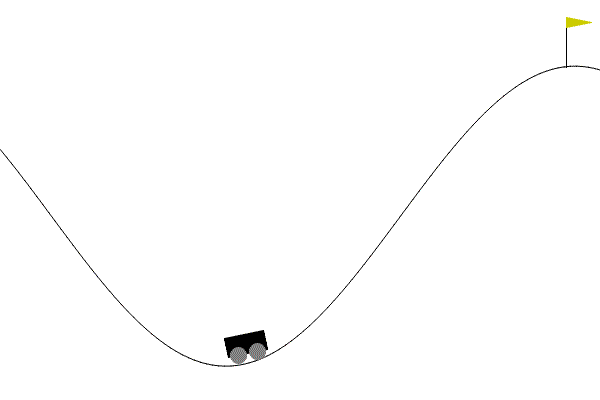
\includegraphics[width=0.4\textwidth]{mountain_car} \hspace*{10mm} 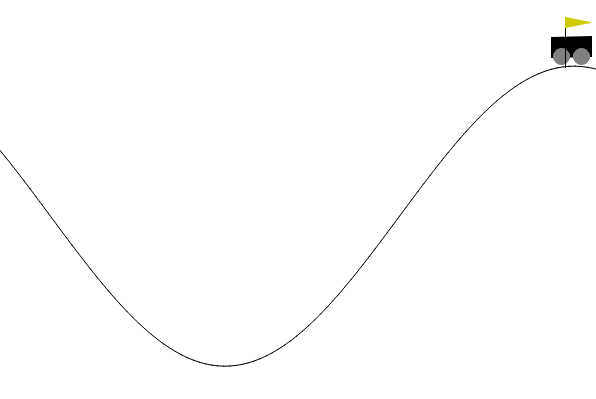
\includegraphics[width=0.4\textwidth]{mountain_car_solved}
\caption[Illustration of the environment MountainCar]{
  \textbf{Illustration of the environments MountainCar and MountainCarContinuous.}
  The image shows one possible state of the environments \texttt{MountainCar} and \texttt{MountainCarContiuous} on the left side. The image on the right shows the target state of the two environments.
}
\label{fig:mountain_car}
\end{figure}

\paragraph*{Action Space:} The action space for the environment \verb|MountainCar| consists of three discrete actions. We can accelerate the car to the right or the left, or we do not interact with it. The actions are further described in Table~\ref{table:mountaincar_act}.
\begin{table}[!ht]
  \centering
  \begin{tabular}{ |c|c|c|c| }
    \hline
    Action & Description & Value & Unit \\
    \hline
    0 & Accelerate to the left & Inf & position(m) \\
    1 & Don't accelerate  & Inf & position(m) \\
    2 & Accelerate to the right  & Inf & position(m) \\
    \hline
  \end{tabular}
  \caption[Action space of the environment MountainCar]{
    \textbf{Action space of the environment MountainCar.}
    Description of all possible actions for the \texttt{MountainCar} environment.
  }
  \label{table:mountaincar_act}
\end{table}
The environment \verb|MountainCarContiuous|, on the other hand, accepts one continuous action per step. The action represents the directional force on the car and is clipped in the range of [-1, 1] and multiplied by a power of 0.0015.

\paragraph*{Observation Space:} The environments \verb|MountainCar| and \verb|MountainCarContiuous| share the same observation space. They return two observations with information about the car's position and velocity. The observations are further described in Table~\ref{table:mountaincar_obs}.
\begin{table}[!ht]
  \centering
  \begin{tabular}{ |c|c|c|c| }
    \hline
    Observation & Min & Max & Unit \\
    \hline
    Position of the car along the x-axis & -Inf & Inf & position(m) \\
    Velocity of the car & -Inf & Inf & position(m) \\
    \hline
  \end{tabular}
  \caption[Observation space of the environment MountainCar]{
    \textbf{Observation space of the environment MountainCar.}
    Description of all observations for the \texttt{MountainCar} and \texttt{MountainCarContiuous} environments.
  }
  \label{table:mountaincar_obs}
\end{table}

\paragraph*{Reward:} To solve the task, the car has to reach the flag on the right hill as fast as possible. Each time step in which the agent cannot get tp the target, it receives a negative reward of -1 for the environment \verb|MountainCar|. For the environment \verb|MountainCarContiuous|, we receive a negative reward of $-0.1 * \text{action}^2$ for each step in which the car does not reach the target to penalize actions of large magnitude. When reaching the goal, we receive a positive reward of +100.

\subsection{Pendulum}
For the environment \verb|Pendulum|, the system consists of a pendulum attached at one end to a fixed point and the other end being free. The goal is to apply torque on the free end to swing it to an upright position. This task is known as the inverted pendulum swing-up problem and is based on the classic problem in control theory. Figure~\ref{fig:pendulum} shows one possible state of the environment in the left image and the target state in the right one.
 \begin{figure}[!ht]
  \centering
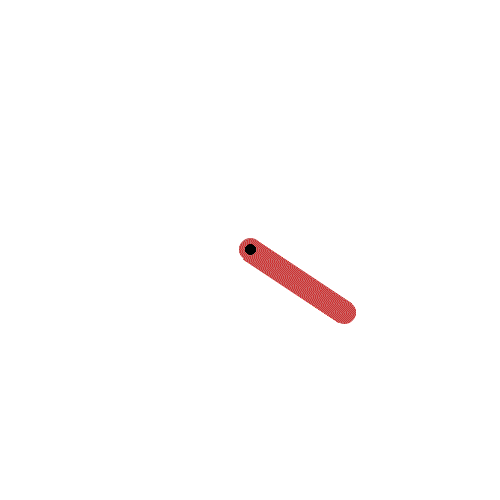
\includegraphics[width=0.4\textwidth]{pendulum} \hspace*{10mm}
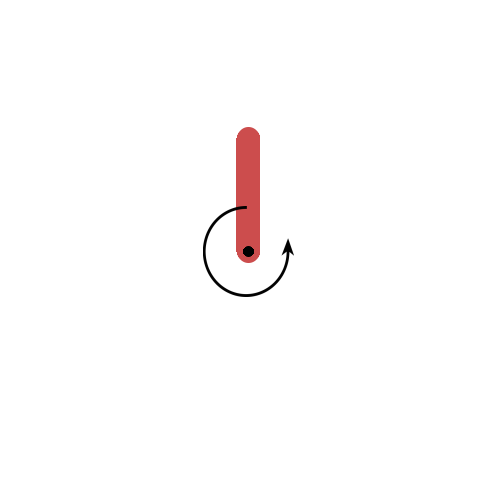
\includegraphics[width=0.4\textwidth]{pendulum_solved}
\caption[Illustration of the environment Pendulum]{
  \textbf{Illustration of the environment Pendulum.}
  The left image shows one possible state of the \texttt{Pendulum} environment. In the right image, the pendulum is in the upright position, which denotes the target state.
}
\label{fig:pendulum}
\end{figure}

\paragraph*{Action Space:} The environment accepts one action per step. The action represents the torque applied to the free end of the pendulum.
\begin{table}[!ht]
  \centering
  \begin{tabular}{ |c|c|c|c| }
    \hline
    Action & Description & Min & Max \\
    \hline
    0 & Torque & -2.0 & 2.0 \\
    \hline
  \end{tabular}
  \caption[Action space of the environment Pendulum]{
    \textbf{Action space of the environment Pendulum.}
    Description of all possible actions for the \texttt{Pendulum} environment.
  }
  \label{table:pendulum_act}
\end{table}

\paragraph*{Observation Space:} The environment returns three observations. The first two observations represent the x- and y-coordinate of the pendulum's free end in a cartesian coordinate system. The variable theta defines the angle in radians. The third observation is the angular velocity of the free end of the pendulum.

\begin{table}[!ht]
  \centering
  \begin{tabular}{ |c|c|c| }
    \hline
    Observation & Min & Max \\
    \hline
    x = cos(theta) & -1.0 & 1.0 \\
    y = sin(angle) & -1.0 & 1.0 \\
    Angular Velocity & -8.0 & 8.0 \\
    \hline
  \end{tabular}
  \caption[Observation space of the environment Pendulum]{
    \textbf{Observation space of the environment Pendulum.}
    Description of all observations for the \texttt{Pendulum} environment.
  }
  \label{table:pendulum_obs}
\end{table}

\paragraph*{Reward:} The reward function is defined as $r$ = -($\text{theta}^2$ + 0.1 * $\text{theta\_dt}^2$ + 0.001 * $\text{torque}^2$). Regardless of the received reward, an episode ends after 200 time steps.

\section{Visualization}
For the visualization of the results, I am using similar plots as \cite{oller_analyzing_2020}. The type of plots I will be using is already presented in Figure~\ref{fig:plots_reproduced}. However, I will mainly be using the scatter plots shown in the middle. Figure~\ref{fig:visualization} shows an example of such a plot.
\begin{figure}[!ht]
  \centering
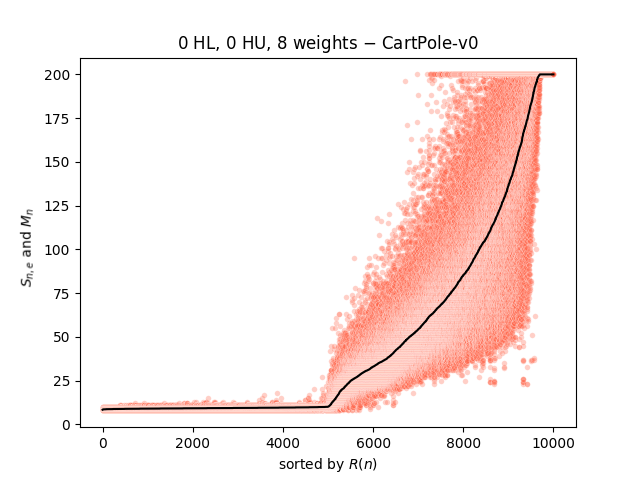
\includegraphics[width=.5\linewidth]{NN/CartPole_NN_HL_0_HU_0_scatter_score.png}
\caption[Visualization of results]{
  \textbf{Visualization of results.}
  The image shows an example of the visualization of the conducted experiments. The scatter plot represents the individual sample scores $S_{n,e}$ for episode $e$ over the rank $R(n)$ of the sample $n$. The overlaid line plot consists of the mean scores $M_n$ for each sample.
}
\label{fig:visualization}
\end{figure}
For a better analysis, the samples are sorted according to their mean score. The position of a sample $n$ within the sorted list is referred to as its rank $R(n)$. In the plot, the samples are aligned according to their rank on the x-axis. Each red dot represents the individual sample score $S_{n,e}$ for sample $n$ in episode $e$. The overlaid line plot represents the mean score $M_n$ of sample $n$ over all episodes. Thus, the line plot is a naturally increasing curve of the mean scores. The scatter plot indicates the variety of scores for one sample. The title of the plot informs us which model and how many weights were used. In addition, the corresponding OpenAI gym environment is declared.

\todo[inline]{Rethink paper section, present plots here for the first time?}

\section{Alternative Models}
\label{sec:models}
This section describes the models I used in the experiments. Since we are using black-box optimization techniques, we have no constraints on the model. Therefore, we can use any function approximator. Note that we are in the field of direct policy search, where we directly search in the search space of policies for a suited approximation.

\subsection{Polynomials}
In mathematics, a polynomial is the sum of powers in one or more variables multiplied by constant coefficients. Given a field $F$, a polynomial in variable $x$ with coefficients in $F$ is a formal expression denoted by
\begin{align*}
  &f(x) = \Sigma_{i=0}^{n} a_i x^i \in F[x], &a_0, ..., a_n \in F, \ \ i \in \mathbb{N},
\end{align*}
where $F[x]$ represents the set of all such polynomials (\cite{fischer2014}, p. 61). The above formula shows the one dimensional case. For the multi-dimensional case, $x$ and the coefficients are vectors instead of scalars. Thus, a polynomial $p(\mathbf{x})$ with $\mathbf{x} = [x_0, ..., x_m]^T$ being a vector and of degree $n$ can be represented by
\begin{align*}
  &p(\mathbf{x}) = \Sigma_{i=0}^{n} \mathbf{w_i}^T (x_k^i)_{k \in I} \in F^n[\mathbf{x}], &\mathbf{w_0}, ... \mathbf{w_n} \in F^n, \ \ I = \{0, ..., m\}.
\end{align*}
Polynomials are relatively simple mathematical expressions and offer some significant advantages: their derivative and indefinite integral are easy to determine and are also polynomial. Due to their simple structure, polynomials can be valuable to analyze more complex functions using polynomial approximations. \textit{Taylor's theorem} tells us that we can locally approximate any $k$-times differentiable function by a polynomial of degree $k$. We call this approximation \textit{Taylor polynomial}. Furthermore, the \textit{Weierstrass approximation theorem} says that we can uniformly approximate every continuous function defined on a closed interval by a polynomial. Other applications of polynomials are \textit{polynomial interpolation} and \textit{polynomial splines}. Polynomial interpolation describes the problem of constructing a polynomial that passes through all given data points. Polynomial splines are piecewise polynomial functions that can be used for spline interpolation.

For the experiments with the polynomial model in Chapter~\ref{ch:experiments}, I constructed the model $P_1$. It consists of one polynomial for each possible action in a discrete action space. The input of the model is the observation of the environment. The dimension of the weight vectors is according to the dimension of the input vector. For example, for the environment \verb|CartPole| with the discrete action space $\{0, 1\}$ and observation $\mathbf{x} = [x_0, x_1, x_2, x_3]^T$, this means that $P_1$ consists of two polynomials:
\begin{align*}
  &p_0(\mathbf{x}) = \Sigma_{i=0}^{n} \mathbf{w_i}^T (x_k^i)_{k \in I} \in \mathbb{R}, &\mathbf{w_0}, ..., \mathbf{w_3}, \mathbf{x} \in \mathbb{R}^4, \ \ I = \{0, 1, 2, 3\} \\
  &p_1(\mathbf{x}) = \Sigma_{i=0}^{n} \mathbf{\hat{w}_i}^T (x_k^i)_{k \in I} \in \mathbb{R}, &\mathbf{\hat{w}_0}, ..., \mathbf{\hat{w}_3}, \mathbf{x} \in \mathbb{R}^4, \ \ I = \{0, 1, 2, 3\}
\end{align*}
In the formulas, $n$ denotes the degree of the polynomial. For the experiments, I used polynomials of degrees one, twp, and three. However, the output of the polynomials has no appropriate upper and lower limit, as illustrated in Figure~\ref{fig:bounds}. That makes it harder to interpret the results reasonably.
\begin{figure}[ht]
\centering
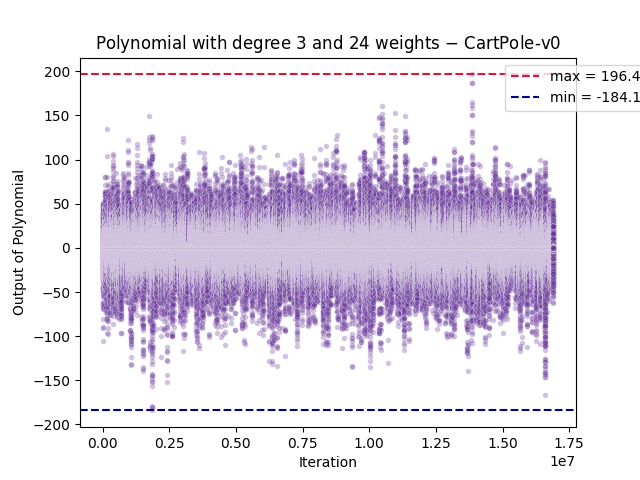
\includegraphics[width=0.6\textwidth]{PolynomialNN_degree_3_bounds}
\caption[Upper and lower bound]{
  \textbf{Upper and lower bound.}
  The figure shows each output of the polynomial functions described above. As we can see, the functions are not well bound, and there are quite a few outliers. That makes it hard to interpret the output sensibly.
}
\label{fig:bounds}
\end{figure}
So, I scaled the outputs with the logistic sigmoid function. We can interpret the output space of the sigmoid function as a probability, as discussed in Section~\ref{subsec:NN}. In this case, we search for the probability that a specific action is the reasonable one given an observation $\mathbf{x}$. Thus, for our example with the \verb|CartPole| environment, we can interpret $sig(p_0)$ as the probability that action 0 is the correct one and $sig(p_1)$ as the probability that action 1 is the correct one. Putting this thought into a formula for $P_1$ and the \verb|CartPole| environment, we get:
\[
  P_1(\mathbf{x}) =
  \begin{cases}1~&{\text{ if }}~sig(p_1(\mathbf{x})) > sig(p_0(\mathbf{x}))~,\\0~&~\text{otherwise}~.\end{cases}
\]

% The second model $P_2$ is constructed similarly to $P_1$, but it only consists of one polynomial instead of one for each possible action. For the \verb|CartPole| environment, this means $P_2$ consists of:
% \[
%   p(\mathbf{x}) = \Sigma_{i=0}^{n} \mathbf{w_i}^T (x_k^i)_{k \in I} \in \mathbb{R}, \ \ \ \ \ \ \ \ \ \ \mathbf{w_i} \in \mathbb{R}^4, \ \ I = \{0, 1, 2, 3\}
% \]
% Analogous to $P_1$, I tested the polynomial $p(\mathbf{x})$ with degrees 1, 2, and 3. So, $n \in \{1, 2, 3\}$. In addition, I again used the logistic sigmoid function to scale the output of the polynomial. However, the output of $P_2$ is determined by a fixed threshold instead of comparing multiple polynomials. Putting this into a formula for the \verb|CartPole| environment, we get:
% \[
%   P_2(\mathbf{x}) =
%   \begin{cases}1~&{\text{ if }}~sig(p(\mathbf{x}))>0.5~,\\0~&~\text{otherwise}~.\end{cases}
% \]

\todo[inline]{Include theorems (Taylor, Weierstass) \\ Explain difference between approximation and interpolation \\ Does $F^n$ make sense?}

\subsection{Splines}
General splines, adjustments \\ \\
Splines can also be used as function approximators. However, with splines we do not aim to approximate the whole function but rather return a piecewise approximation.

\todo[inline]{First was sind splines, dann herleitung in this case.}


\subsection{Binary Trees}
A binary trees are data structures in computer science with a rather simple structure. The tree consists of nodes that each have at most two children, referred to as left child and right child.

\begin{figure}[!ht]
\centering
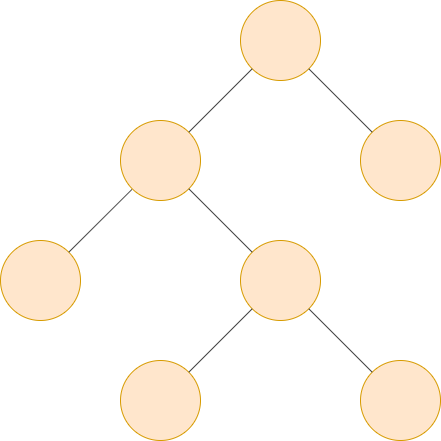
\includegraphics[width=0.4\textwidth]{binary_tree}
\caption[Example of a binary tree]{
  \textbf{Example of a binary tree.}
  The figure shows an example of a binary tree with seven nodes.
}
\label{fig:binary_tree_illustration}
\end{figure}

There exist already some tree-based machine learning algorithms. However, they are mostly used in supervised learning.
% https://medium.com/analytics-vidhya/tree-based-machine-learning-algorithms-explained-b50937d3cf8e

\todo[inline]{Herleitung von splines erklären -> vielleicht in vorheriger subsection? Explain continuous envs.}
